\documentclass[10pt]{article}
 
\usepackage[margin=1in]{geometry} 
\usepackage{amsmath,amsthm,amssymb, graphicx, multicol, array}
\usepackage{parskip}
 
\newcommand{\N}{\mathbb{N}}
\newcommand{\Z}{\mathbb{Z}}
 

\begin{document}
 
\title{Problem Set 1}
\author{Nicolas Morales, Kushal Patel, Olivia Wilkinson \\
ECON: 880}
\maketitle

\section{Problem 1}

The execution time for the un-parallelized implementation takes about 63 seconds while the parallelized implementation finishes in about 20 seconds. 

\section{Problem 2}
\begin{figure}[!h]
    \centering
    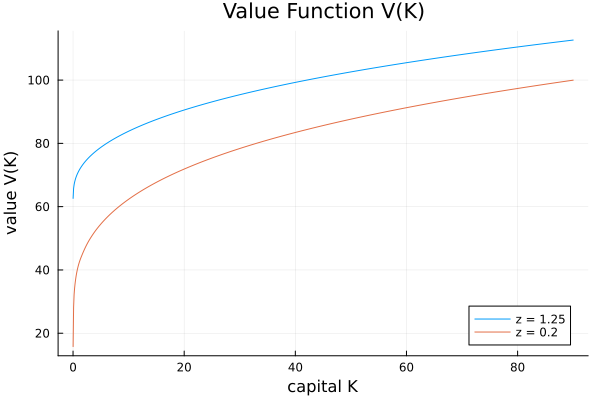
\includegraphics[width = 0.65\textwidth]{Value_Functions.png}
\end{figure}

The value function is plotted for both states $z = 1.25$ and $z = 0.2$. The value function is clearly increasing and concave. 

\newpage 
\section{Problem 3}
\begin{figure}[!h]
    \centering
    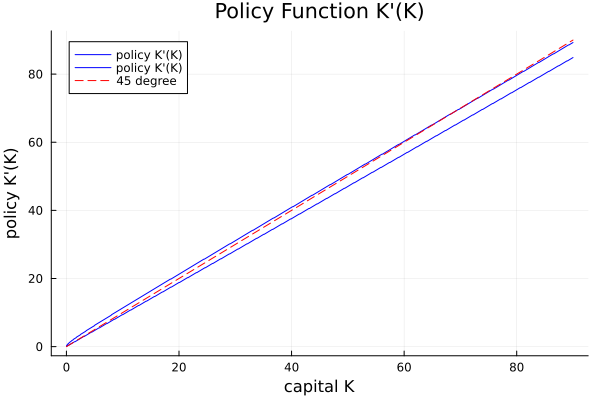
\includegraphics[width = 0.49\textwidth]{Policy_Functions.png}
    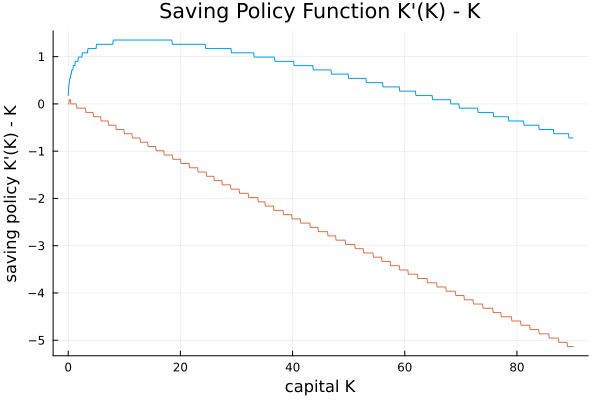
\includegraphics[width = 0.49\textwidth]{Policy_Functions_Changes.png}

\end{figure}

The policy function is clearly increasing in $K$. Since $K'(K, Z_{h})$ lies above $K'(K, Z_{l})$ , it is also increasing in $Z$. Savings is increasing in $Z$. When productivity is high, savings is increasing in $K$ for low values of $K$ but then decreasing. When productivity is low, savings is monotonically decreasing. 

The euler equation is given by 
\[ \underbrace{\frac{1}{c_t}}_{\substack{\text{marginal utility} \\  \text{of consumption}}} = \underbrace{\beta \mathbf{E}_t \left[ \frac{\alpha z_{t+1} k_{t+1}^{\alpha - 1} + 1 - \delta }{c_{t+1}} \right]}_{\text{marginal cost of saving}} . \]

The LHS captures the marginal utility of consuming more while the RHS is the marginal cost of foregoing consumption today for consumption in the future. When $K$ is low, households might save more in response to a positive productivity shock since they can capture higher future returns. When $K$ is high, a positive productivity shock
leads to increased consumption since they have a lot of wealth and the MPK is low at high $K$. This explains the non-monotonic shape of the savings curve above for high TFP. On the other hand, a negative productivity shock decreases the MPK of capital and disincentivizes savings. 

\end{document}
